
%------------------------------------------------------------------------------
\section{\disr{} Overview}
%------------------------------------------------------------------------------

\label{sec:disr_concepts}
The main concept behind the kind of turn prohibition we want to
achieve is the \emph{segment}. A segment $S_y$ is basically a path of consecutive
nodes and links, starting with a link attached to a node belonging to
a different segment $S_x$ and ending with a link attached to a
node of another segment $S_z$. In other words, a segment is
a path connecting two other different segments. The example
in Figure~\ref{fig:segments} shows the segment with id $1.4$, starting
with a link connected to the node $9$, traversing nodes
$4$, $3$, $2$ and ending with the link connected to the node $1$. Other
segments depicted are, for example, $9.2$ (link from $9$, node $10$, link to node $3$) and $9.3$
(link from $9$, node $8$, link, node $7$, link, node $6$, link, node $5$, link to node $1$). Note
also that start/ending links can coincide and a segment can also be
formed by one single link (e.g. the case of $7.2$ and $5.4$).
An exception to the rule that a segment must connect two other
segments is the first segment established in the network, called
\emph{starting segment} which is a loop beginning/ending on the same
node.

\begin{figure}
\centering
    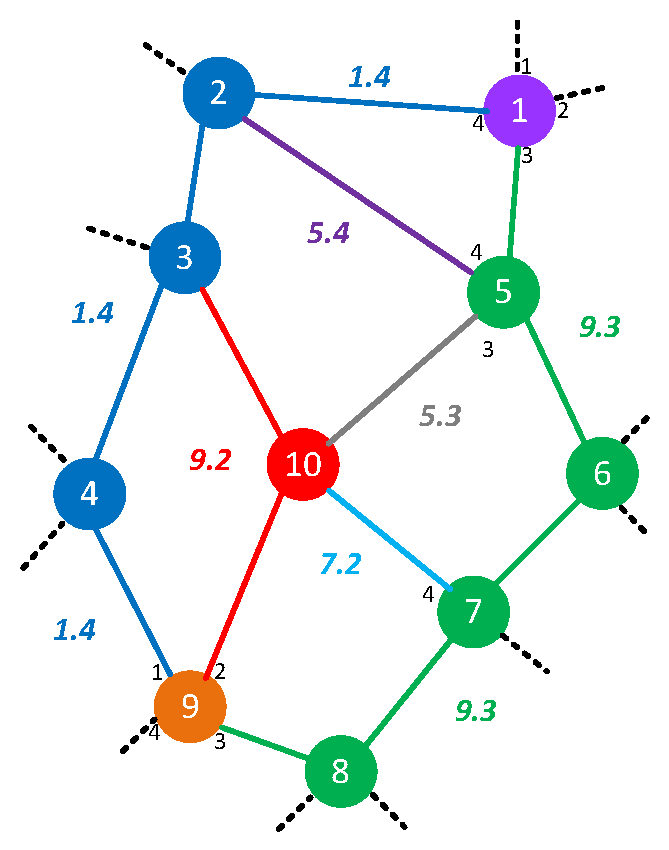
\includegraphics[width=0.25\textwidth]{pictures/network_slice.eps}
  \caption{Example of Segments}
  \label{fig:segments}
\end{figure}

A detailed description of the \disr{} execution model as depicted in
Figure~\ref{fig:disr_events} will be discussed in
Subsection~\ref{sub:phases}. Roughly speaking, the execution phases consist of:
\begin{enumerate}
\item Injection of the \disr{} process from an upper layer to set a \emph{bootstrap
node}.
\item Broadcasting and confirmation to create the first segment of the subnet.
\item Parallel requests starting from assigned node to discover other
segments. 
\item Turn prohibition in each confirmed segment.
\item Draining of remaining packet due to timeouts.
\end{enumerate}

\subsection{\disr{} Data Structures}
\label{ssec:disr_data}

We distinct between two different kinds of data stored in each node:
\emph{Dynamic Behavior Status} (\emph{DBS}) and \emph{Local
Environment Data} (\emph{LED}).

\hl{The \emph{DBS} stores information in order to capture the dynamic
behavior of the node in the context of the whole
\disr{} execution phased.| \emph{DBS} information represent node's status and are related to the current execution phase}. 
The \emph{DBS} can have the following values:

\begin{itemize}
\item{\emph{Free}}: a node that has  not been yet considered  by the \disr{} algorithm.
\item{\emph{Bootstrap}}: a node which has been explicitly set as bootstrap node from
an upper layer via. 
\item{\emph{ActiveSearching}}: a node from which a new segments searching process has
been started and not yet cancelled or confirmed. 
\item{\emph{Candidate}}: a node currently candidate to be part of a segment, but not being itself the node from which the searching process was started. 
\item{\emph{CandidateStarting}}: same as above, but the node is currently being considered as candidate
for starting segment. 
\item{\emph{Assigned}}: a node for which the segment has been determined.  
\end{itemize}

The \emph{LED} are a kind of instant snapshot of the execution of \disr{} algorithm, taken in each node,
consisting in the following variables:

\begin{itemize}
\item{\emph{segID}}: a value used to specify the segment to which the
node has been assigned or is currently candidate to be part of.
\item{\emph{visited}}: a boolean value. When \emph{true}
then a \emph{segID} different from \texttt{NULL} specifies the segment 
to which the node has been assigned. 
\item{\emph{tvisited}}: a boolean value. If \emph{true}, the node is
being considered as candidate for a segment, and the \emph{segID} value
specifies the segment id for which the node is candidate. 
\item{\emph{link\_visited[]}}: an array
of values representing information about attached links, that is, the
segID of the segment owning each link. When \texttt{NULL}, the corresponding link has not yet been
assigned.
\item{\emph{link\_tvisited[]}}: an array of
values representing information about attached links, that is, the \emph{segID} of
the segment for which the link is candidate. When \texttt{NULL}, the link is
not candidate for any segment, i.e. it has already been assigned or it is free.
\end{itemize}

\subsection{Message Types Required}

The \disr{} approach works with a distributed mechanism which is build
upon an exchange of small packets containing the following fields:
\begin{itemize}
\item \emph{packet\_type}: encodes the meaning of the control packet.
\item \emph{seg\_ID}: \hl{the id of the segment associated to the \disr{} control message}.
\item \emph{src\_id}: the id of the node that originated the packet.
\end{itemize}

For what concerns\emph{packet\_type} field, we can have the following control packets types:
\begin{itemize}
\item{\texttt{STARTING\_SEGMENT\_REQUEST}}: Injected by the bootstrap
node when searching the first segment. 
\item{\texttt{STARTING\_SEGMENT\_CONFIRM}}: used when establishing
the starting segment. 
\item{\texttt{SEGMENT\_REQUEST}}: used to search candidates for a segment (\hl{which is} not the
first)
\item{\texttt{SEGMENT\_CONFIRM}}: used to establish a segment. 
\item{\texttt{SEGMENT\_CANCEL}}: used to cancel the process of searching a segment along a
specific link.
\end{itemize}

A quantitative analysis of the resources needed to implement and
manage these structures is presented in Section~\ref{sec:implementation} where is discussed 
the impact of \disr{} control logic and storage on the
node's hardware implementation.

\subsection{Execution Model}
\label{sub:phases}

The \disr{} control packets described in the previous subsection trigger
node events, which \hl{eventually} change $DBS$ status according to the
current value of $LED$ variables and the type of packet received.
The main \disr{} phases, together with a reference to the particular
status transition involved are described in the following. As a
convention, we used single letters to refer to one of the \emph{DBS} transitions in
Figure~\ref{fig:state_machine} while the phases are visually
represented in~\ref{fig:disr_events}.

\begin{figure}
  \centering
    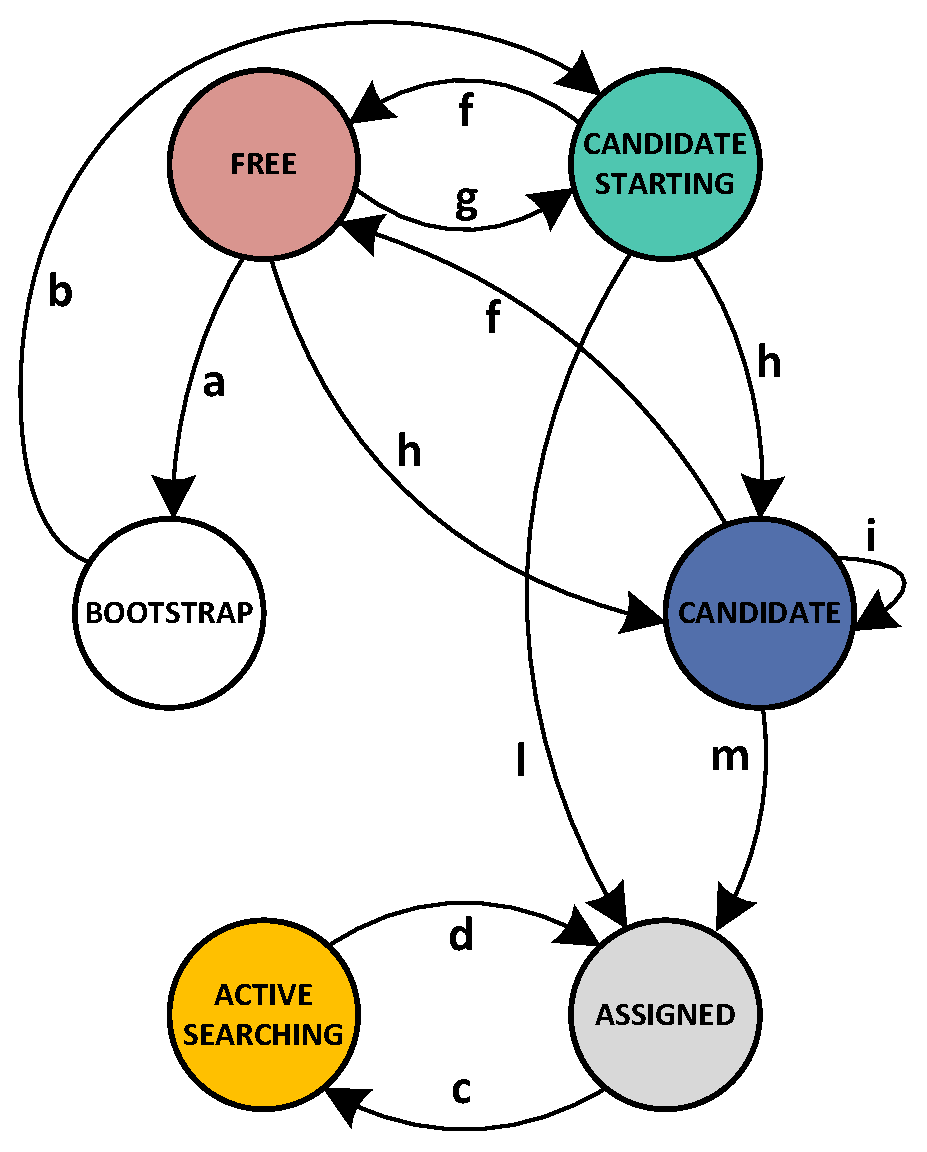
\includegraphics[width=0.25\textwidth]{pictures/dbs_updated.eps}
  \caption{\disr{} node execution model}
  \label{fig:state_machine}
\end{figure}

\begin{figure*}
\centering
\begin{tabular}{cccc}
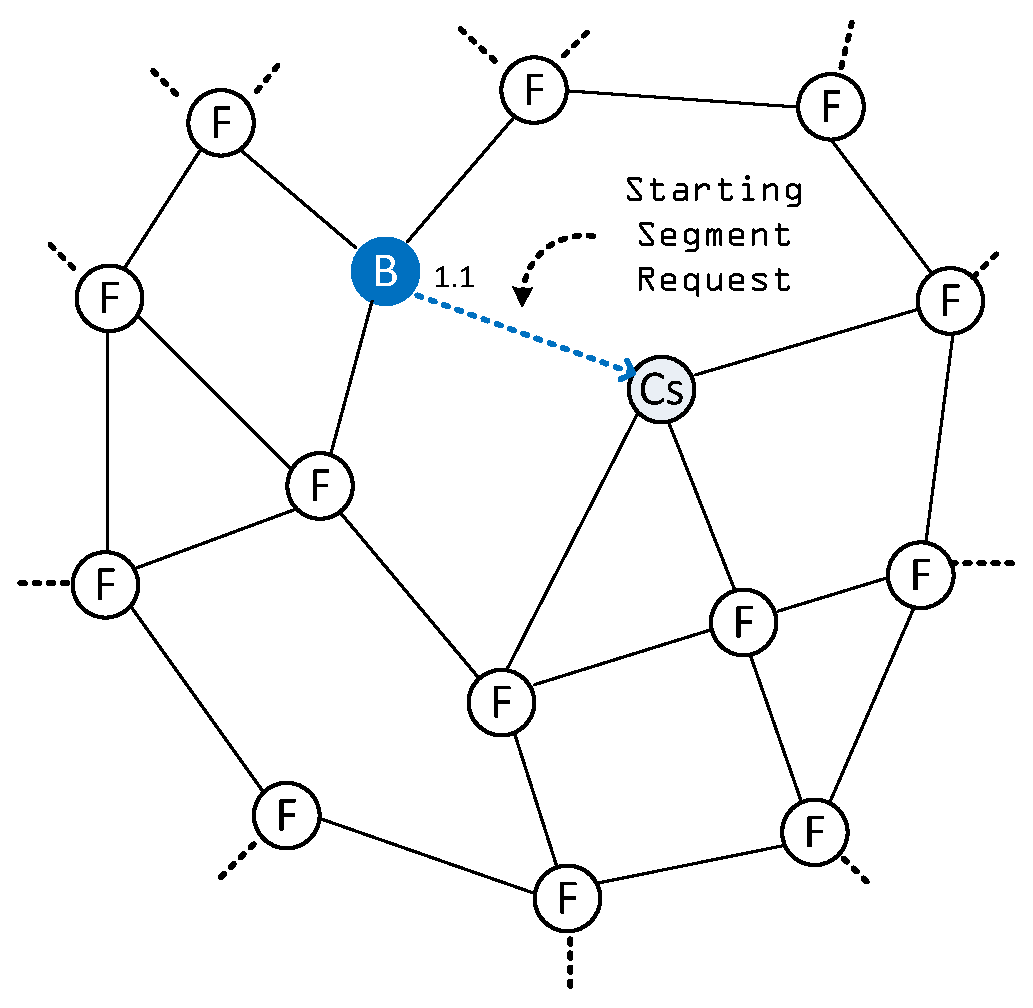
\includegraphics[width=0.23\textwidth]{pictures/seq01.eps} & 
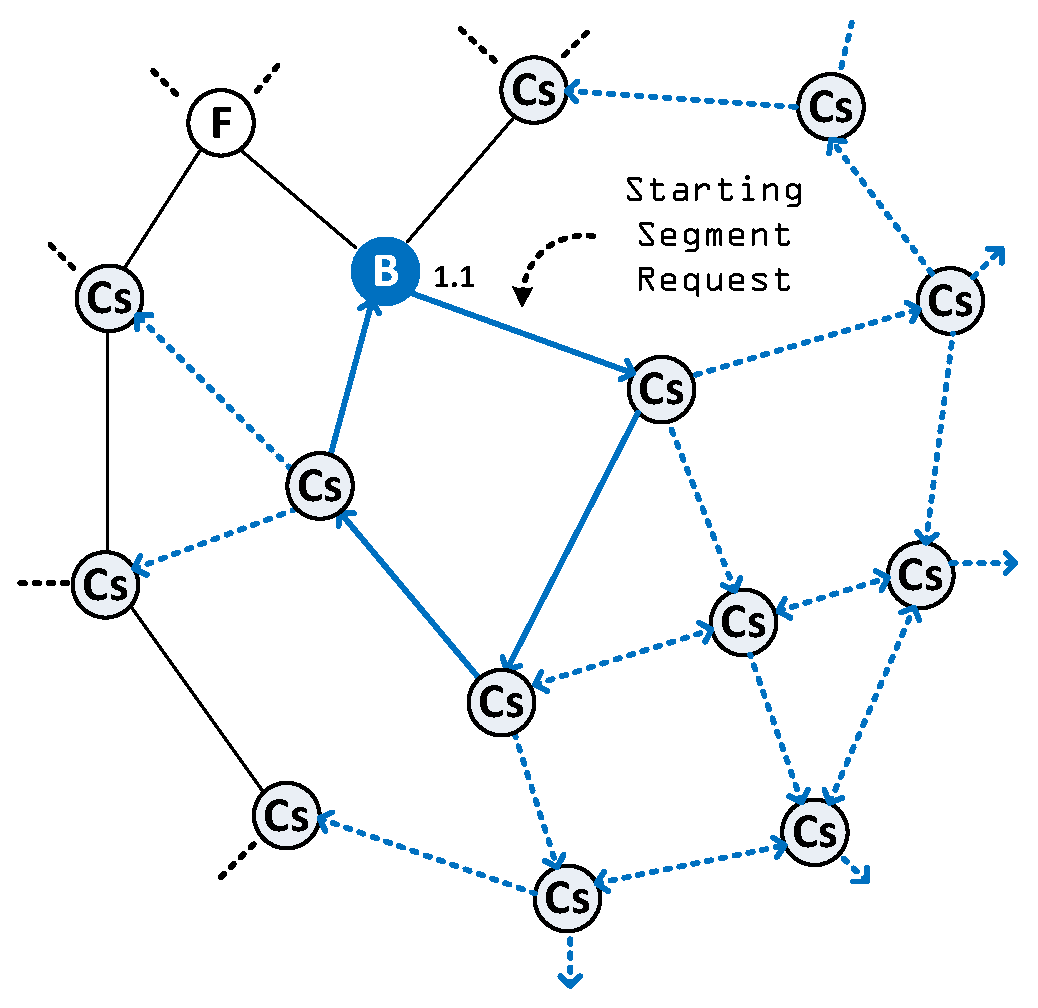
\includegraphics[width=0.23\textwidth]{pictures/seq02.eps} &
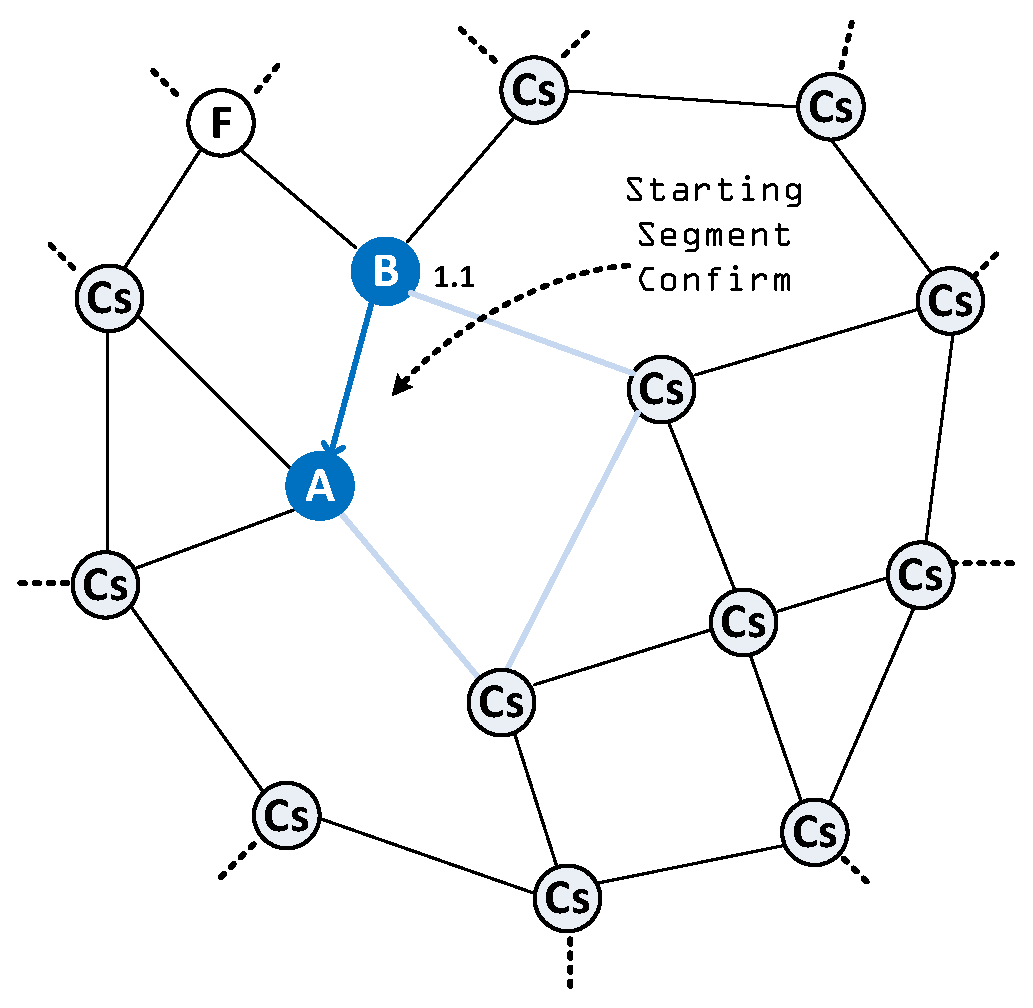
\includegraphics[width=0.23\textwidth]{pictures/seq03.eps} & 
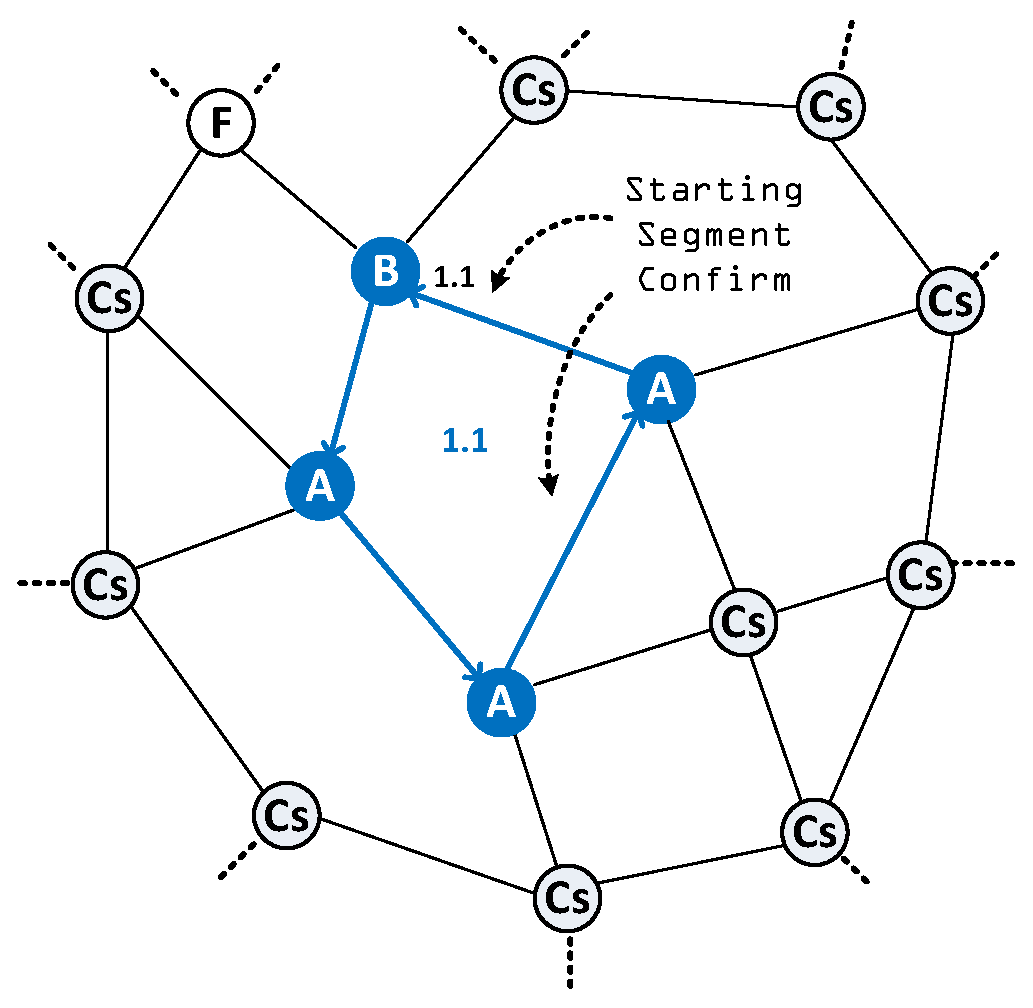
\includegraphics[width=0.23\textwidth]{pictures/seq04.eps} \\
(a) & (b) & (c) & (d) \\
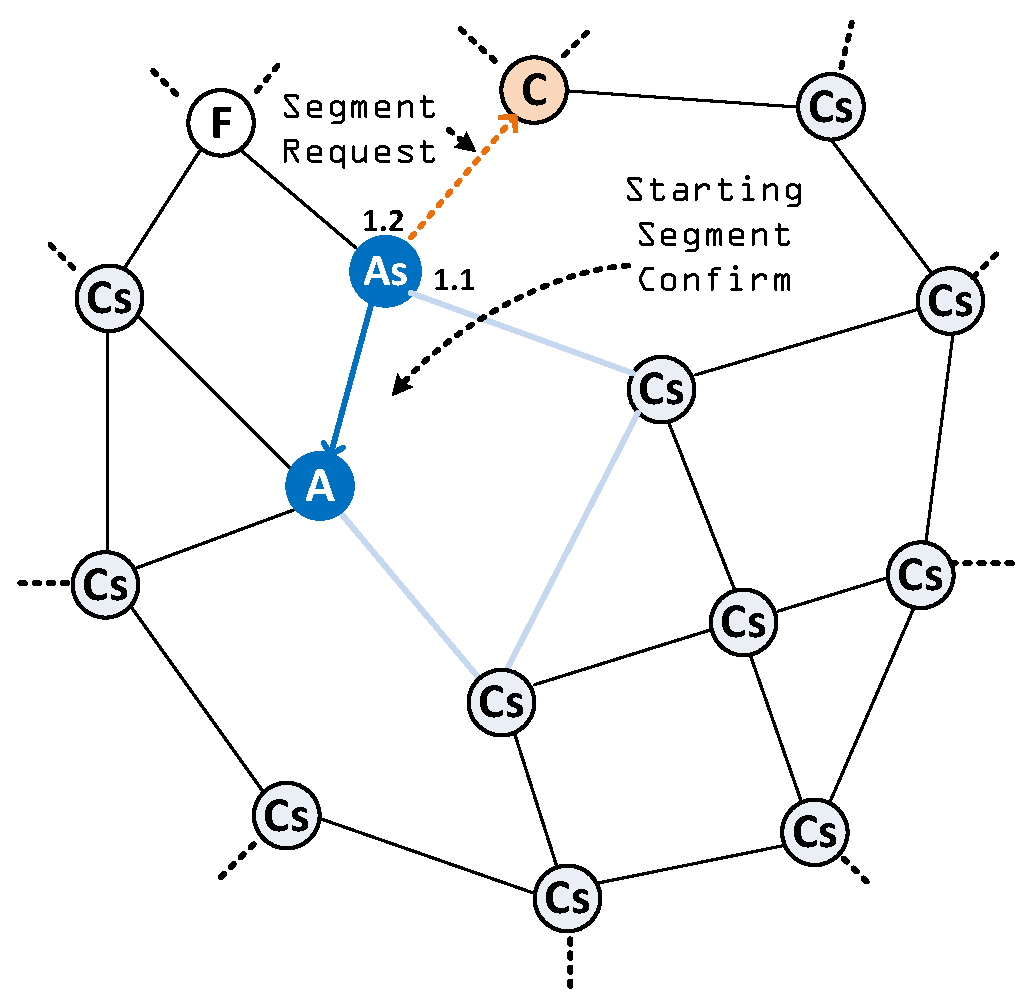
\includegraphics[width=0.23\textwidth]{pictures/seq05.eps} &
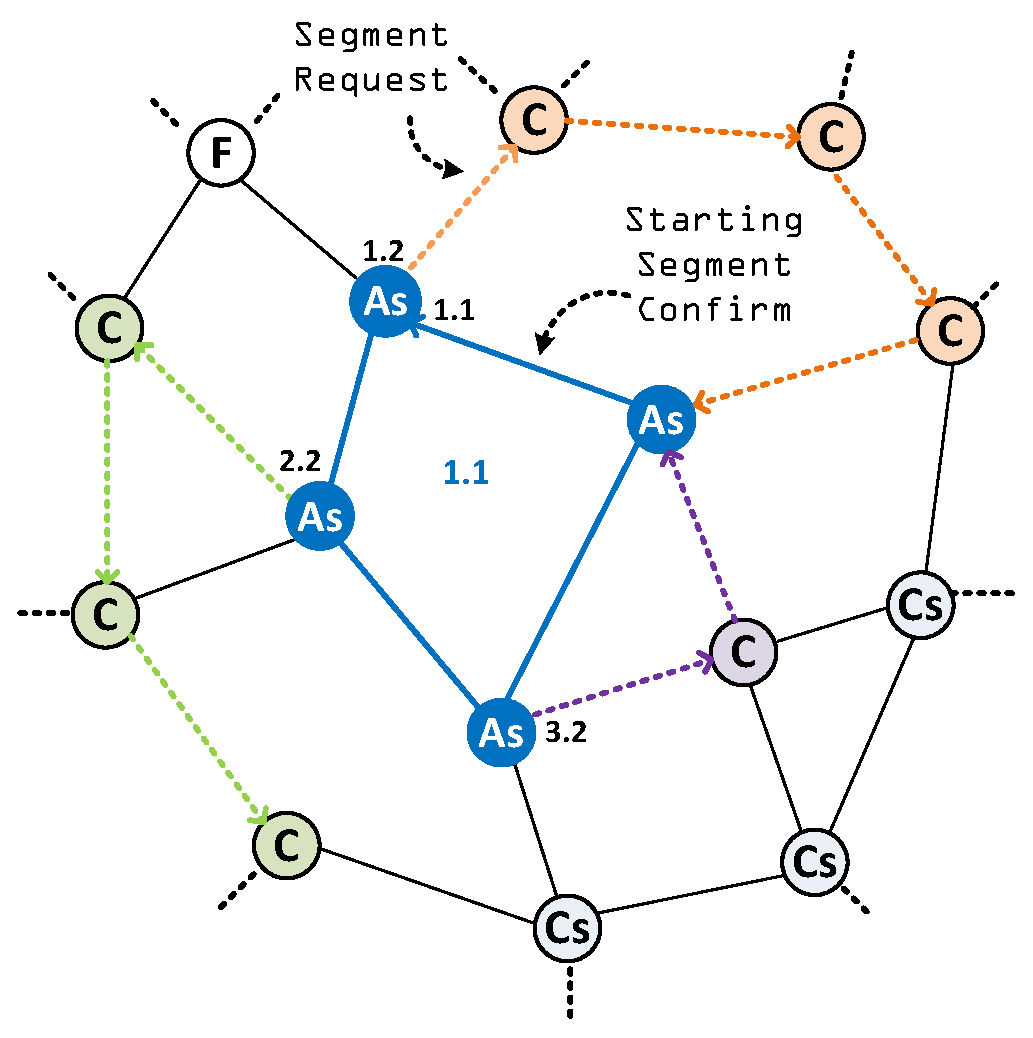
\includegraphics[width=0.23\textwidth]{pictures/seq06.eps} &
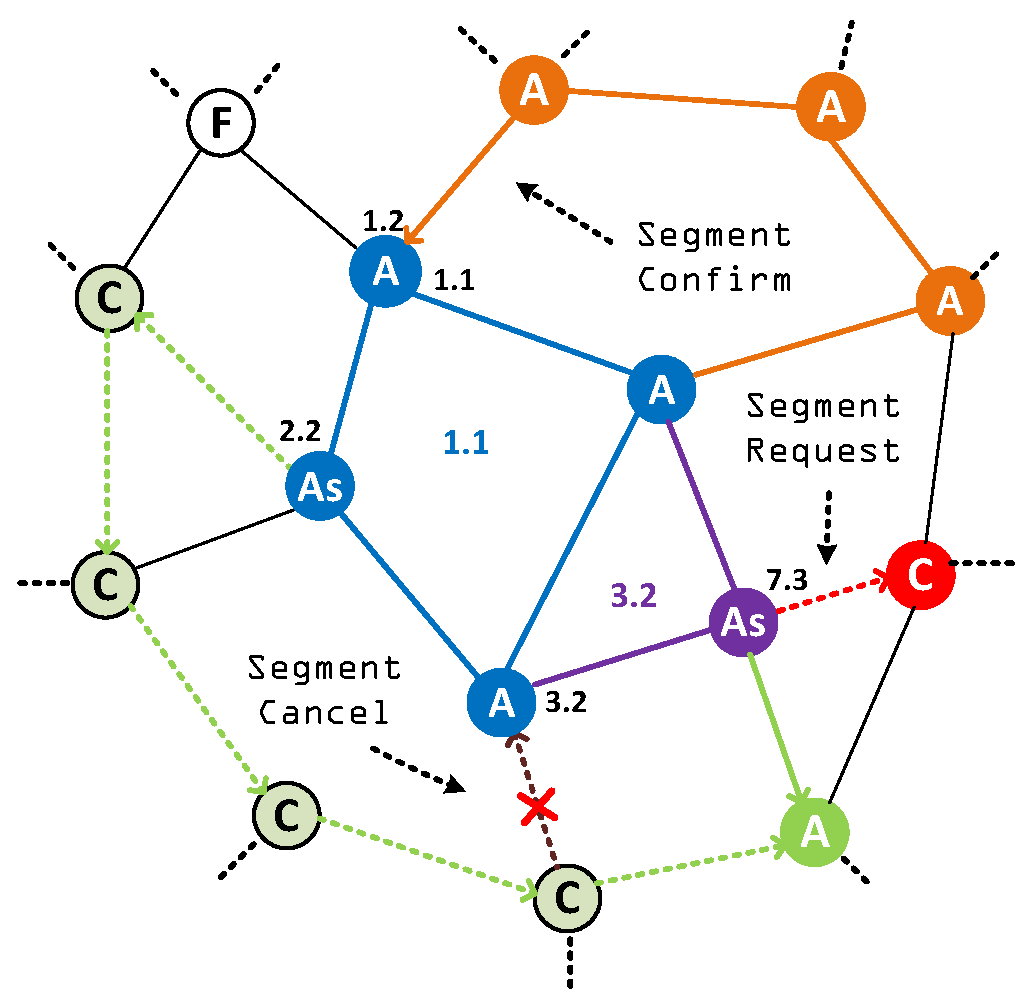
\includegraphics[width=0.23\textwidth]{pictures/seq07.eps} & 
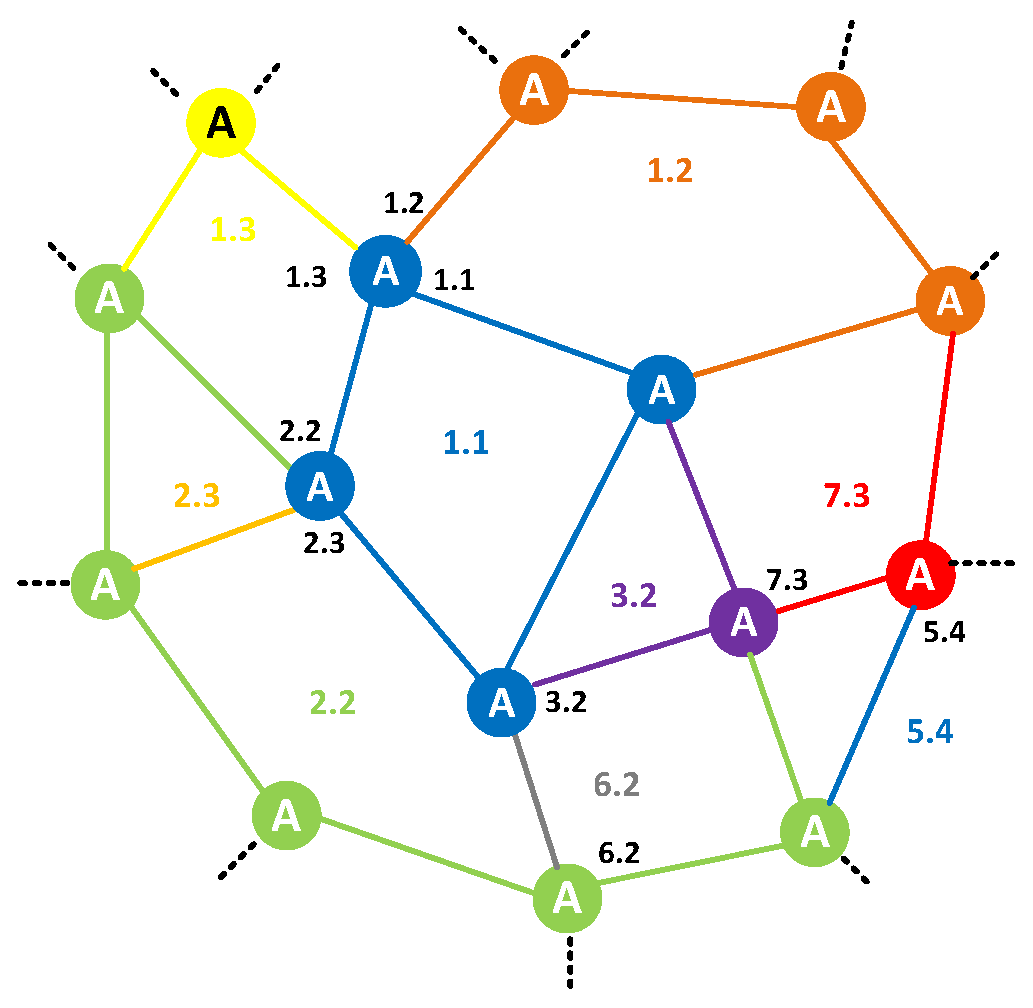
\includegraphics[width=0.23\textwidth]{pictures/seq08.eps} \\
(e) & (f) & (g) & (h) \\
\end{tabular}
\caption{Example of \disr{} segment setup: Nodes' status is labeled as CandidateStarting($Cs$), Candidate ($C$), Free ($F$), Assigned ($A$) or Bootstrap ($B$)}
\label{fig:disr_events}
\end{figure*}

\begin{itemize}
\item{\textbf{Injecting bootstrap request}}: all nodes have an initial
\emph{DBS} status set to \emph{Free}, except for a
 node with status \emph{Bootstrap}, set by some control signal from an
upper layer via $(a)$. When starting, this bootstrap node 
changes its status to \emph{CandidateStarting} $(b)$, injecting a
\texttt{STARTING\_SEGMENT\_REQUEST} across one of its free links
(Figure~\ref{fig:disr_events}-a). 

\item{\textbf{Bootnode Broadcasting}}: Each node receiving a \texttt{STARTING\_SEGMENT\_REQUEST},
when $Free$, forwards it to its free links using a flooding mechanism and
becoming $CandidateStarting$ $(g)$.
Each of its free links is then marked as \emph{tvisited} with the segment id
associated to the request. Note that a node that has already received a
\texttt{STARTING\_SEGMENT\_REQUEST} packet can simply ignore further packets
associated to the same request, having already contributed to the
flooding (Figure~\ref{fig:disr_events}-b).
%Note also that each of these packets has a max\_segment\_hops
%field to prevent packets from traveling undefinitively.  

\item{\textbf{Confirming the Starting Segment}}: when a \texttt{STARTING\_SEGMENT\_REQUEST} packet reaches
the bootstrap node (from a different link, of course), the starting
segment is found. Then the bootstrap node sends back a \texttt{STARTING\_SEGMENT\_CONFIRM}
packet along the link from which it received the
\texttt{STARTING\_SEGMENT\_REQUEST} and becomes \emph{Assigned} $(l)$. Each
node receiving the confirmation does the same by changing its own status
to \emph{Assigned}(Figure~\ref{fig:disr_events}-c). So the confirmation packet is sent back from
node to node and the starting segment is created (Figure~\ref{fig:disr_events}-d). 


%What happens to nodes not receiving these segment request?
%they simply remain \emph{tvisited} and after a timeout reset their
%state as free. But they could also remain \emph{tvisited} for the
%starting segment, since this does not affect their behavior for future
%segment requests.  

%failure: TODO should we handle this case ? i.e.  marking as terminal ?

\item{\textbf{Injecting Segment Requests}}: Each node in the
\emph{Assigned} status can potentially initiate a new segment request.
So it check its links and if a free link is found it changes its
status to $ActiveSearching$ $(c)$ and then sends
a \texttt{SEGMENT\_REQUEST} across the free link $(c)$ (see
Figure~\ref{fig:disr_events}-e). 
Note that each \emph{Assigned} node can inject the request just after
becoming \emph{Assigned}, i.e. it is not needed that the whole confirmation
process in completed (Figure~\ref{fig:disr_events}-f).
Note also that nodes previously set as \emph{CandidateStarting}, when receive
a \texttt{SEGMENT\_REQUEST} can simply cancel their
status and set themselves as $Candidate$ for that request, since this new
request means that the first starting segment has already been found $(h)$. 
\item{\textbf{Segment Confirmation}}: The segment searching process is successful
when an already \emph{Assigned} node receives the
\texttt{SEGMENT\_REQUEST} packet. Then, a \texttt{SEGMENT\_CONFIRM} is
sent back along the path that originated the request
(Figure~\ref{fig:disr_events}-g), while the
node remains $Assigned$ \hl{(since it could confirm more segments)}. Each node
previously set as $Candidate$ for that segment id, when receives a confirmation packet changes its status to \emph{Assigned} $(m)$ and send back
the same confirmation until it reaches the initiator of the request,
which then changes from $ActiveSearching$ to $Assigned$ $(d)$.

\item{\textbf{Failing while searching a segment}}: this happen when a node receives a \texttt{SEGMENT\_REQUEST} packet but
matches one of two the following conditions: the node is $Free$ but has no
more suitable free links (thus can’t forward the
\texttt{SEGMENT\_REQUEST})$(f)$; the node
is already \emph{Candidate} with another segment id, i.e. is part of another searching process. In all these cases the node
sends back a \texttt{SEGMENT\_CANCEL} along the incoming link (see at
the bottom of Figure~\ref{fig:disr_events}).
\end{itemize}


\section{Detailed Node Behavior Model}
\label{sec:execution_model}

In this Section we provide further details about \disr{}
execution model, describing the internal behavior implemented in
each node. Note that this also corresponds exactly to what should be
implemented from the \hl{node-hardware} perspective, as discussed in
Section~\ref{sec:implementation}.

The \emph{LED} variables in each node
($segID$, $visited$, $tvisited$, \emph{link\_visited[]}, \emph{link\_tvisited[]})
are initially set as \texttt{NULL}, so the node and all its links
are considered as \emph{Free}.
The only node that makes an exception is the bootstrap node, initialized
in the \emph{Bootstrap} status. All the subsequent events happening at
each node are the consequence of its current dynamic status (DBS), the
packets received and the internal status represented by the
\emph{LED}. Note that in the following, when using expression like
``has a free link'' or ``free node'' we will assume the relationship between 
$LED$ and $DBS$ discussed in Section~\ref{ssec:disr_data}. Further, for
each packet type all the cases not explicitly listed can simply be
ignored since are associated to invalid/inconsistent events of the
\disr{} execution model. A complete list of these cases can be checked
in the environment simulator source code at~\cite{nanoxim}.

\subsection{Receiving a \texttt{STARTING\_SEGMENT\_REQUEST}}
The request for the first segment should be managed differently since
all nodes (except the bootstrap one) must forward the packet using a
broadcasting mechanism. This is necessary since the request packet must
return the bootstrap node.
When a node receives a \texttt{STARTING\_SEGMENT\_REQUEST}, the
following cases can happen:

\begin{itemize}
\item The node is $Free$: it should set itself as
\emph{CandidateStarting} and forward the packet along its free links, using
broadcasting and marking these links as $tvisited$ with $segID$ found
in the packet.
\item The node is \emph{CandidateStarting} with the same
\emph{segID} and \emph{src\_id} of the packet is equal to the node id:
this means that the node was the initiator of the request, thus a starting segment has
just been found and should be confirmed sending back a \texttt{STARTING\_SEGMENT\_CONFIRM}
packet.  
\item The node is \emph{CandidateStarting}, with the same \emph{segID} of the
packet but the \emph{src\_id} field is different from the node id: since the node is candidate with the same id, it means
that it already accomplished the task of propagating that kind of
packets, thus can simply ignore the event dropping the packet.  
\item The node is \emph{Candidate}, with a different \emph{segID}: 
this simply means that the \texttt{STARTING\_SEGMENT\_REQUEST} just received is deprecated,
because the node has already accepted a non-starting segment request originated from another \emph{Assigned} node.
\item The node is \emph{Assigned}, with a different \emph{segID}:
same as the previous case. 

% TODO: check and remove, the below is not true
%CHECK:  it is not the initiator of the starting segment request, but
%is already assigned to some segment!? assuming again we are discussing
%of nodes belonging to the same subnet, this should NOT happen, since
%the only visited node of the subnet should be the initial node from
%which the \texttt{STARTING\_SEGMENT\_REQUEST} originated. Note again that we are
%assuming that if the the node is visited or \emph{tvisited} with the id of
%another subnet can simply ignore the request.  The node is \emph{tvisited}
%but it is not the initiator of the request (different id): same as
%above, if we are assuming nodes of the same subnet, this should not
%happen. If the node is of another subnet, can simply ignore the event.

\end{itemize}

\subsection{Receiving a \texttt{SEGMENT\_REQUEST}}
When a node receives a \texttt{SEGMENT\_REQUEST}, there are the following cases:

\begin{itemize}
\item The node is \emph{Assigned}: a segment should be confirmed
sending back a \texttt{SEGMENT\_CONFIRM} packet.
\item The node is \emph{Candidate}: it should discard the packet sending
back a \texttt{SEGMENT\_CANCEL}.
\item The node is \emph{Free} and has free
links: it marks itself as \emph{Candidate} and forwards the \texttt{SEGMENT\_REQUEST}
to one of its free links, according to some internal ordering.
\item The node is \emph{CandidateStarting}: same as being $Free$,
since a segment request circulating in the network indicates that the
starting segment process has been completed.
\end{itemize}

Note that the main difference between confirming a \texttt{STARTING\_SEGMENT\_REQUEST}
and confirming a \texttt{SEGMENT\_REQUEST} is that in the first case the node
itself is included in the segment.

%The motivation is
%that in the second case the node was already marked as \emph{visited} because
%of being assigned to some segment found before, while in the
%starting-segment case, by definition, the first segment of a subnet
%begins with the starting node, which is marked as \emph{visited} by the SR
%algorithm when searching the first (starting) segment. Remember
%that the first segment of a subnet is a loop beginning with the
%starting node. 

\subsection{Receiving a \texttt{SEGMENT\_CONFIRM}}
When the node status is \emph{Candidate} with a \emph{segID} corresponding to the one indicated in
the packet: the node set itself as $Assigned$ to the segment $segID$. Further, it should forward this packet to the link where the
original \texttt{SEGMENT\_REQUEST} packet came from, so that all candidate nodes
can learn the id of the segment they belong to. Then, \emph{LED} should be
updated from \emph{tvisited} to \emph{visited}.

\subsection{Receiving a \texttt{SEGMENT\_CANCEL}}
When a node receives a \texttt{SEGMENT\_CANCEL} packet it means that the research
for a segment along that path was unsuccessful. But if the
node still has some other free link to try, it should forward a
\texttt{SEGMENT\_REQUEST} to the those links. So a node forwards back
the \texttt{SEGMENT\_CANCEL} packet along the link that originated the
\texttt{SEGMENT\_REQUEST} packet $only$ when there are no more free
links to try. If this is the case, the node modifies its status from
\emph{Candidate} to \emph{Free} and forwards the
\texttt{SEGMENT\_CANCEL} packet to the link from which the request was
received. The process stops when the \texttt{SEGMENT\_CANCEL} packet
reach the starting node that originated the request.

\subsection{Intra-node vs Inter-node parallelism}
In the processes described above, we assumed that each node in the
\emph{Assigned} status can start a segment searching process by injecting a
\texttt{SEGMENT\_REQUEST}. However, a more accurate decision when
defining \disr{} should be made in order to decide whether or not the
node must actually perform this action. The point above is
strictly related to a general question: which level of
parallelism should we allow in \disr{}? The adopted approach, although
the nature of \disr{} itself is intrinsically parallel, is that the use of
parallelism makes things working in a more complex way. In other words,
\disr{} is parallel when needed, but it does not exploit parallelism
as an ``improving feature''. When not needed, things should be
serialized. For example: when a node is ``ready to search'' it could start
several segment searching processes associated to the same segment, one for
each free link. But serializing this operation, by investigating the free links
in order, could be a simpler solution. We refer to this saying that we
avoid intra-node parallelism.  Note that while intra-node parallelism
can be avoided, trying to avoid inter-node parallelism could be more
complex than allowing the parallelism itself. Imagine for example the
effort generated trying to coordinate nodes so that an unique segment searching
process is actually running in the whole subnet. Thus, in contrast to
the intra-node parallelism, the inter-node parallelism is a structural
property of the \disr{} algorithm and should not be avoided.
%------------------------------------------------------------------------------
